This chapter gives an overview about the Online Access Law regarding its regulations, their implementation, the basic OZG use case and the underlying system architecture.

\subsection{Regulations}

In 2017, the German government passed the Online Access Law (OZG) which requires federal republic and member states to execute the following regulations until 2022 \cite{BMI:OZG_Wortlaut}:

\paragraph{Digital availability of administrative services} An administrative service is the electronic processing of administrative procedures that are available from outside the governmental institution.  As it is not clear which administrative services exactly are included by the definition of the OZG, the Federal Ministry of the Interior Building and Community (Bundesministerium des Innern, für Bau und Heimat - BMI) created a catalogue \cite{BMI:Verwaltungsleistungen}. The OZG requires these services to be digitally available. As a guideline to what is considered sufficient availability, the BMI defined a maturity model \cite{BMI:Digitale_Services}.

\paragraph{Digital access to administrative services through administration portals of a portal network} Federal republic, each federal state and each commune must provide an administration portal. Portals of communes must be linked to the portal of the corresponding member state. Portals of federal republic and member states must be connected through a portal network. \cite{BMI:Portalverbund} Each portal must provide a "seek and find" feature, which enables users to find all administrative services provided by any administration portal \cite{Cotar:Drucksache_19/19089}. 

\paragraph{Interoperable user profiles for accessing administrative services} Federal republic and member states must provide user profiles that can be used to identify the corresponding person while requesting access to administrative services, to save personal information according to the once-only principle, to receive and send messages via a digital mailbox and to pay for services \cite{Cotar:Drucksache_19/19089}. The user profiles must be interoperable for every administration portal of the portal network.

\subsection{Implementation of Regulations}

The implementation of OZG regulations can be separated into two projects: The digitalization and the networking project.

The goal of digitalization in this case is, to make administrative services available towards a user in a digitized way: A digitized administrative service can be accessed by a user through a website. The website is hosted either by the federal republic or a federal state and is called "Administration Portal". Access is usually provided through an application form. The administrative service can be managed through a user profile which is provided by the federal republic or the member state. Management of an administrative service usually includes starting the service by sending in a form, communicating with the responsible institutions through the inbox of the profile and receiving a result. The user profile can also enable users to upload documents to a datawallet and to save personal information for automatically filling in forms.

Digitalization of an administrative service is the modification of the underlying processes to incorporate the usage of the described features of the user profile and administration portal. In total, the BMI lists 575 relevant services, some of them provided by the federal republic, some by the member states and some by the communes \cite{BMI:Onlinezugangsgesetz}.

The networking focuses on connecting governmental systems to make all digitized administrative services available for every user. This includes most importantly the connection of administration portals to a portal network through an online gateway and the interoperability of user profiles.

In order to save investments a method called "one for all" is used when hosting administrative services. One federal state or the federal republic provides access to a service on their administration portal and distributes the requests to the responsible institutions "under the hood". As administration portals are connected through an "online gateway", each portal contains a search feature, which enables users to find all administrative services through any portal. Interoperable user profiles enable usage of each profile for management of administrative services on all portals.

\subsection{Basic Use Case}
Each time users apply for administrative services, they have to go through an application process, in the following section summarized as the basic OZG use case.

A user wants to apply for two administrative services: funding under the Federal Training Assistance Act (BAföG) and a drivers license. Both administrative services are provided through the "one-for-all" method. The federal state Sachsen-Anhalt is responsible for processing BAföG applications on its administration portal and the federal state Hessen is responsible for processing drivers license applications on its administration portal. The user has never access OZG services before.

\paragraph{Create User Profile} The user wants to apply for BAföG first and therefore visits an administration portal which informs them, that in order to apply for administrative services, a user profile is required. As user profiles are designed to be interoperable, it does not matter through which administration portal the user profile is created.

The user is requested to enter personal information and to specify an authentication method. For authentication for example a username and password combination can be used.

\paragraph{Selection of Administrative Service} Using the search feature of the administration portal, the user enters the search term "bafög" and is presented with a list of administrative services as result. The user selects the correct administrative service from the search result and is forwarded to the web page of the service on the administration portal of Sachsen-Anhalt . It contains information about the administrative service along with instructions on how to access an interactive application form which is can be hosted on a separate web page.

\paragraph{Login to User Profile} Before being able to apply for administrative services, the user has to login into the user profile on the administration portal. Depending on the authentication method used for logging in, a trust level of the current session is determined. Only with a high trust level users can apply for a broad selection of administrative services. The user has selected an authentication method which results in a high trust level.
    
\paragraph{Application} On the web page of the administrative portal the user clicks on a "bring me to the application" button and is forwarded to a web page with an interactive form. Before the user is forwarded, he has the option to transfer personal information for automatic filling of the form. The user decides to accept and is presented with a filled in form. After pressing the "submit" button the application is transferred to the responsible institution.
    
\paragraph{Management of Applications} The user is forwarded back to the administration portal and selects to view all active applications created through the portal. Here the user can see the application they just submitted and is able manage it by for example requesting cancellation.
    
\paragraph{Communication} Through the inbox of the user profile the user is notified about a message regarding the application. The institution responsible for processing the application informs the user about receiving the application. Eventually the institution finishes processing the application and sends a message to the inbox of the user to inform them about the result. This marks the end of the basic OZG use case, however, the user wants to apply for a second administrative service.

\paragraph{Selection of Administrative Service} Using the search feature of the administration portal, the user now enters the search term "drivers license", selects the correct search result and is forwarded to the corresponding web page on the administration portal of Hessen. 

\paragraph{Login to User Profile} The same interoperable user profile can be used as on the administration portal of Sachsen-Anhalt, but the user is required to login again.

\paragraph{Application} The application process is designed to be similar for each administration portal, however, as Sachsen-Anhalt and Hessen operate their application processes independently, minor differences exist in for example the design and text of the web pages.

\paragraph{Management of Applications} The user is, again, forwarded back to the administration portal and selects to view all active applications created through the portal. The user is only able to see and manage the application for a drivers license. As the application for BAföG was created through a the administration portal of Sachsen-Anhalt, it is not accessible through the administration portal of Hessen.

\paragraph{Communication} Through the inbox of the user profile, the responsible institution again sends notifications about the current status and results of the application.

\subsection{System Architecture}
This section describes the OZG system architecture of a federal state capable of executing the basic OZG use case. References about OZG system architectures of Baden-Württemberg \cite{ozg:bw} and Nordrhein-Westfalen \cite{ozg:nrw} are used. The presentation document regarding the administration portal of Baden-Württemberg \cite{ozg:bw_administration_portal} is used as basis for describing the administration portal.

As shown in figure \ref{ozg:system_overview}, the OZG system architecture is separated into three components and two domains. Domains in this case separate systems in regard to the physical location where they operate. Components in this case describe functionally correlated systems of a system architecture.

The "User Component" directly interacts with users to enable access to administration portals. This can be desktop or mobile applications or as in this specific case a web browser. The "Administration Portal Component" hosts the administration portal. The "User Profile Component" provides interoperable user profiles. The "Integration Component" transfers filled in applications to responsible institutions. And finally, the "Institution Component" receives and processes applications.

\begin{figure}[h]
    \centering
    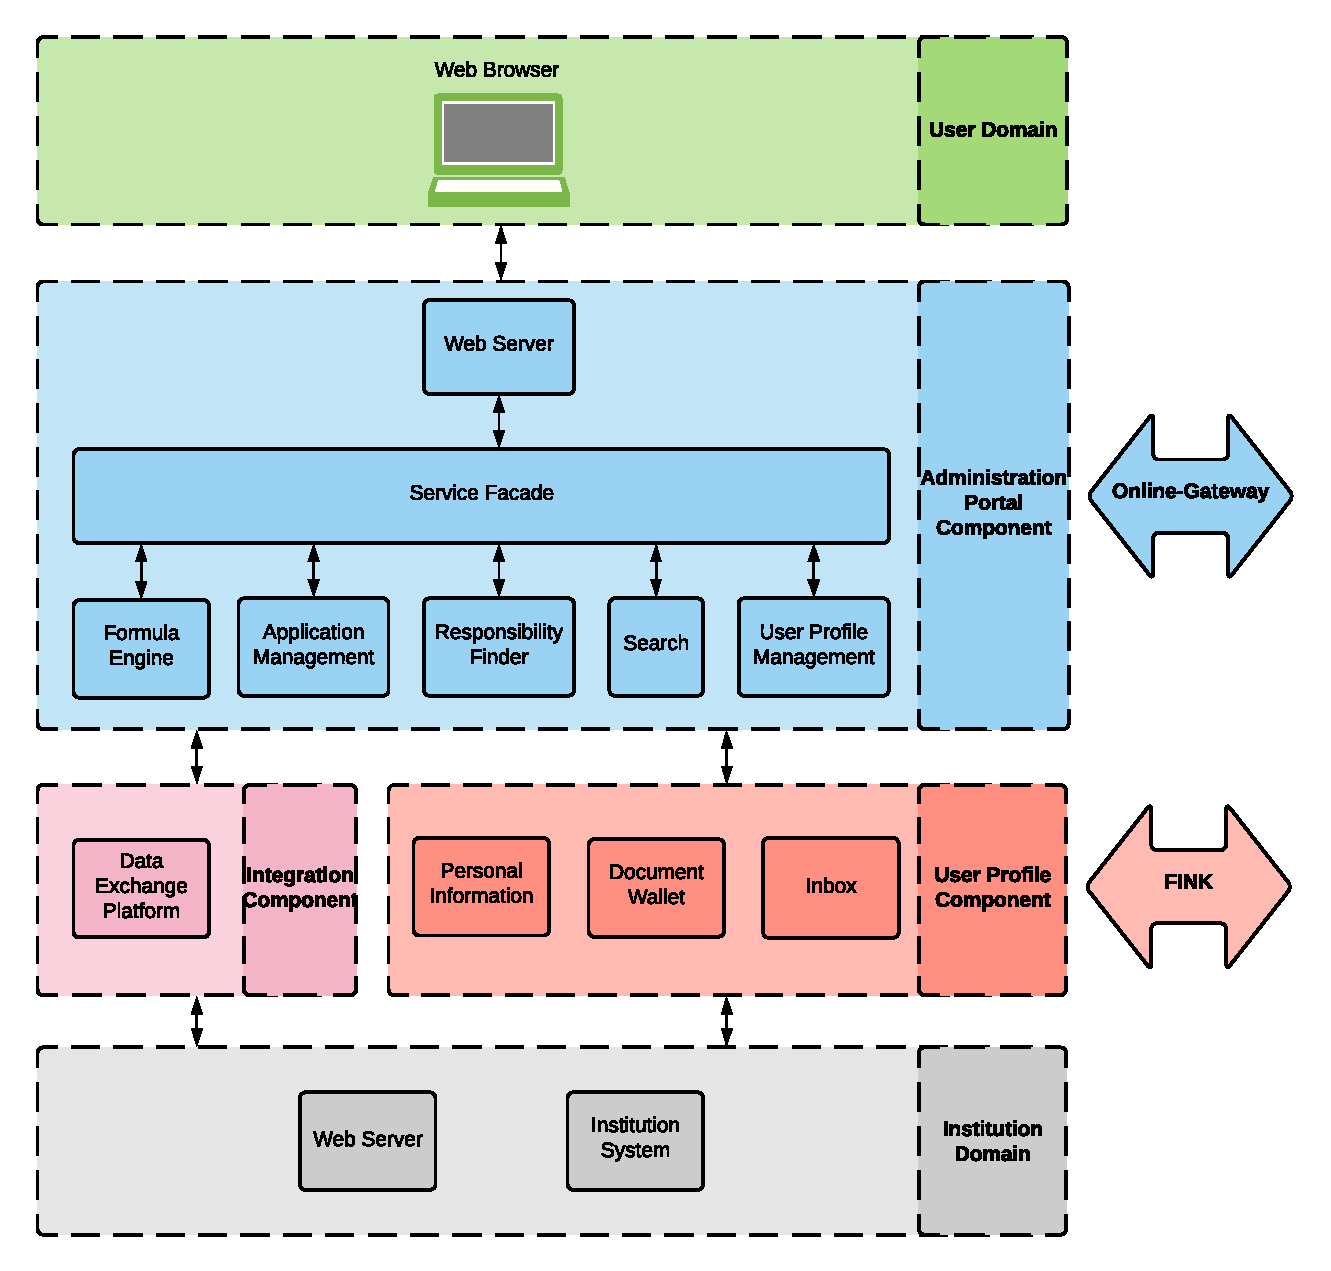
\includegraphics[scale=0.6]{Diagrams/OZG System Overview.pdf}
    \caption{OZG System Overview}
    \label{ozg:system_overview}
\end{figure}

The administration portal directly interacts with the "User Component" through a web page and provides access to the basic OZG use case by interacting with other components. It consists of a web server that is responsible for hosting web pages and a service facade connected to multiple service components. Through the service facade, the web server accesses each service component and makes its service available to the "User Component". 
The "User Profile Management" component is capable of interacting with the "User Profile Component" to create new user profiles, retrieve personal information from existing user profiles and process login requests. 
The "User Profile Component" provides conventional user profile based identity management. 
Through the Federated Identity Management of Interoperable User Accounts in Germany (Föderiertes Identitätsmanagement interoperabler Nutzerkonten in Deutschland - FINK) the "User Profile" component of each federal state is made interoperable. The "Search" component can be used to retrieve a list of URLs of administrative services corresponding to a search term. It can retrieve URLs of administrative services from all administration portals through the "Online-Gateway".

The "Online-Gateway" is a system connecting all administration portals and enabling them to exchange information. The "Formula Engine" component is accessed by the web server to display interactive forms to the user when applying for selected administrative services. The interactive form can be either integrated into the web page of the administrative service or hosted on a separate web page. The user can opt in to automatically fill in forms with personal information. In that case, after authentication of the user, the "Administration Portal" component retrieves personal information from the "User Profile" component and sends it to the "Formula Engine" before displaying a filled in form to the user. 

The "Application Management" component receives submitted applications by the "Formula Engine" component for further processing. Depending on the administration portal and type of application, additional processing steps, that are not part of the use case can take place. This includes for example payment processes. The component tracks the current status of the application which the user can view through the web page of the administration portal. It is also capable of terminating the application process if the user requests it. 

The "Application Management" component sends information about the application to the "Responsibility Finder" component which returns an identification of the institution responsible for processing the application. Along with the institution ID, the "Application Management" component submits the application to the "Data Exchange Platform". This component transfers the application data to the institution corresponding to the specified institution ID. The institution can register their "Institution System" to automatically receive the application from the "Data Exchange Platform" where it will be processed. In addition to that, the "Institution Component" hosts a web page with information about the institution.